\documentclass[]{article}
\usepackage[utf8]{inputenc}
\usepackage[a4paper]{geometry}  \geometry{hmargin=1.5cm,vmargin=1.5 cm}
\usepackage{xcolor}
\usepackage{amsmath}
\usepackage{amssymb}
\usepackage{amsfonts}
\usepackage{booktabs}
\usepackage{amsthm}
\usepackage{array}
\usepackage{epsfig}
\usepackage{caption}
\usepackage{empheq}
\usepackage{multicol}
\captionsetup{position=below}
\setlength{\parindent}{0pt}
\usepackage{graphicx}
\usepackage{color}
\usepackage{fancybox}
\usepackage{listings}
\usepackage{hyperref}
\usepackage{euscript}
\usepackage{float}
\usepackage{cite}


\theoremstyle{plain}
\newtheorem{theorem}{Théorème}
\newtheorem{lemma}[theorem]{Lemme}
\newtheorem{corollary}[theorem]{Corollaire}
\newtheorem{proposition}[theorem]{Proposition}
\newtheorem{example}[theorem]{Exemple}

\theoremstyle{remark}
\newtheorem{remark}{Remarque}

\begin{document}

\begin{center} 
	\huge Figures annex
\end{center}

\section{Simuation sketch}

\begin{figure}[h]
	\begin{center}
		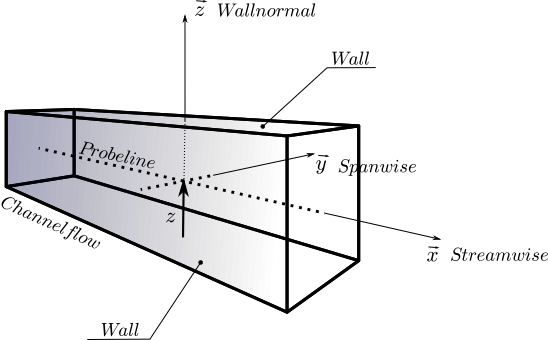
\includegraphics[width=\textwidth]{../../report/referance/channel_flow.png}
		\caption{Sketch of the simulation}
	\end{center}
\end{figure}

\section{RANS and LES comparison}

\begin{figure}[h]
	\begin{center}
	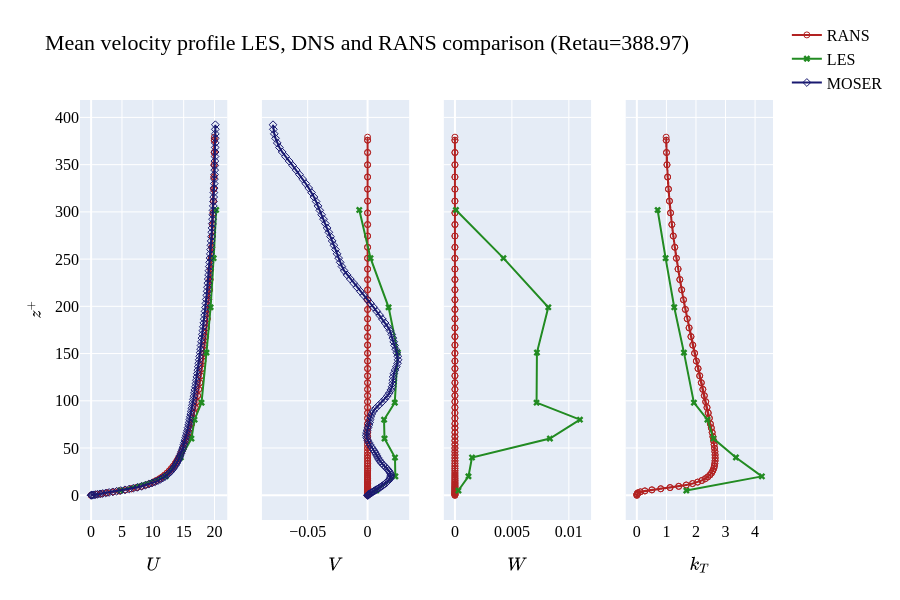
\includegraphics[width=\textwidth]{../../output/figures/channel_wrles_retau395/split_time/RANS/RANS_LES_MOSER_profiles_all.png}
	\caption{The comparison between RANS and LES data profiles of streamwise velocity (left figure) and kinetic energy (right) in function of $z^+$}
	\end{center}
\end{figure}



\section{Velocity analyses}


\begin{figure}[H]
	\begin{center}
		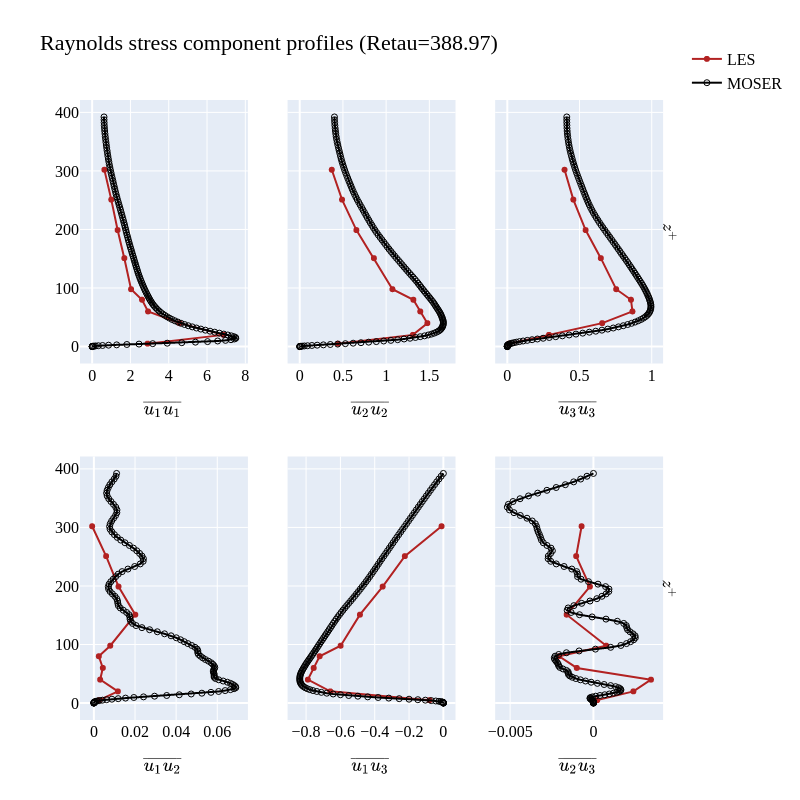
\includegraphics[width=\textwidth]{../../output/figures/channel_wrles_retau395/split_time/RANS/var_velocity_profiles_all.png}
		\caption{Three variance velocity fluctuation profiles from LES datas extract from 10 streamwise plan.}
	\end{center}
\end{figure}



\begin{figure}[H]
	\begin{center}
	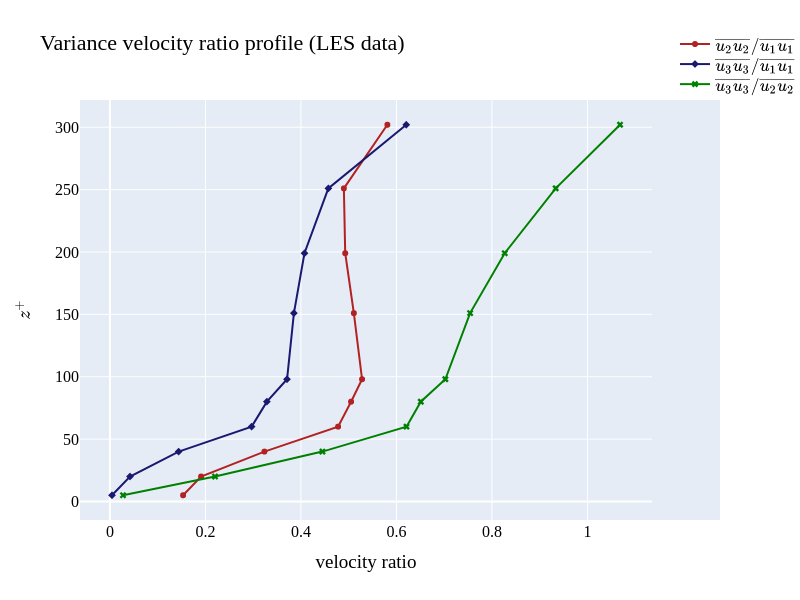
\includegraphics[width=\textwidth]{../../output/figures/channel_wrles_retau395/split_time/RANS/velocity_ratio_profiles_all.png}
	\caption{Square ratio of the spanwise on streamwise velocity (red) and the wall-normal on streamwise velocity (blue). They have been calculated taking the 10 streamwise plans. The streamwise velocity appears to be very dominant on both the spanwise and the wall-normal velocity.}
	\end{center}
\end{figure}



\section{Frozen turbulence}

We want to verify the frozen turbulence hypotethis which state that $\phi_{ij}^{[1]}(k_1,x_2,x_3)=U_c\psi_{ij}(U_ck_1,x_2,x_3)$ with $\omega=U_ck_1$. $U_c$ is the mean streamwise velocity, $\phi_{ij}^{[1]}$ is the spatial spectra in the streamwise direction and $\psi_{ij}$ is the time spectra.

\subsection{2D correlation}

\begin{figure}[H]
	\begin{center}
		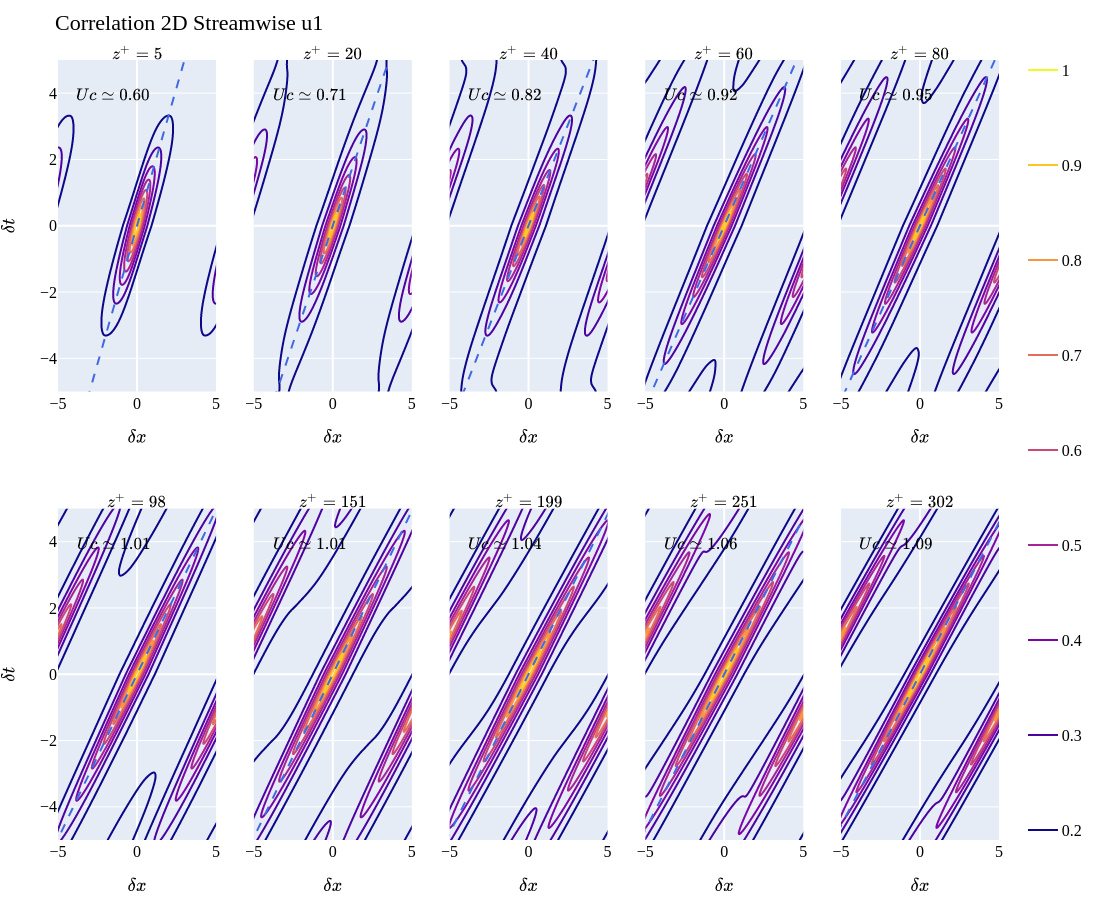
\includegraphics[width=\textwidth]{../../output/figures/channel_wrles_retau395/split_time/frozen_turbulence/correlation2D/u1_all.png}
		
	\end{center}
\end{figure}

\begin{figure}[H]
	\begin{center}
		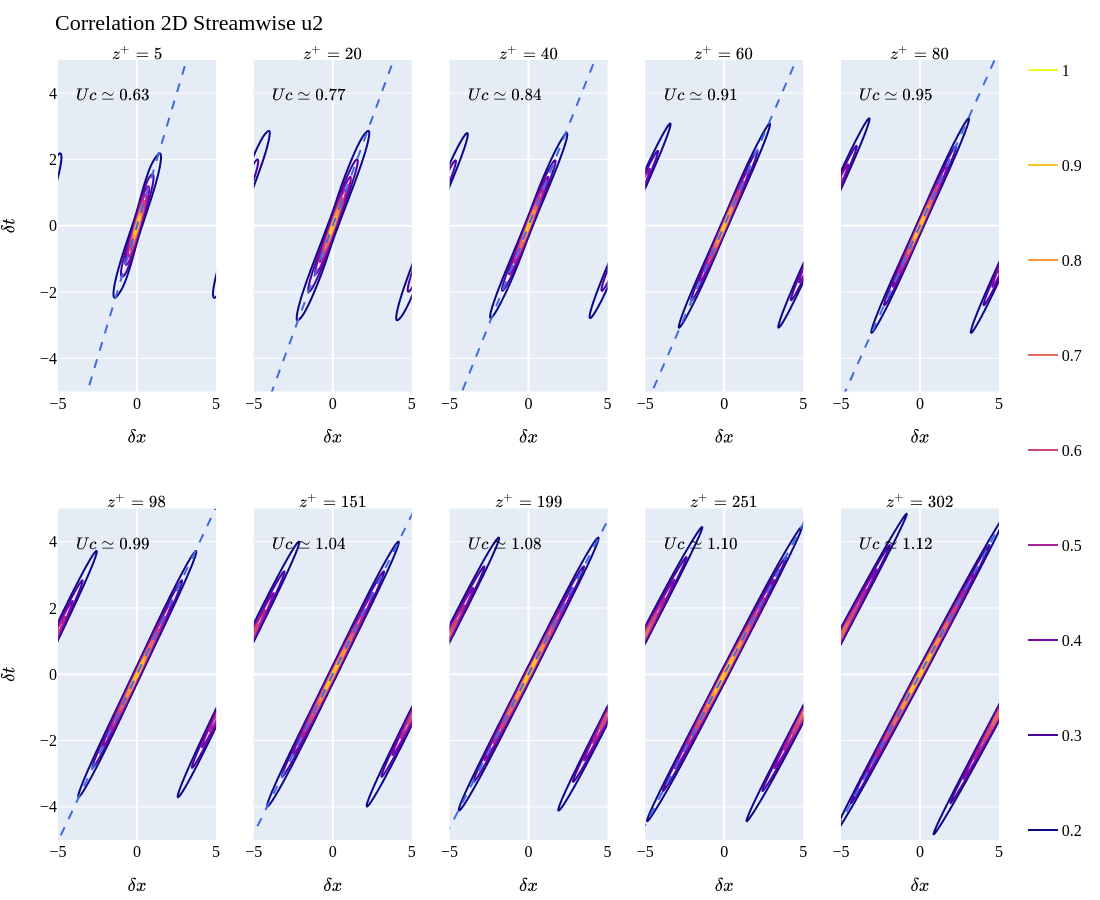
\includegraphics[width=\textwidth]{../../output/figures/channel_wrles_retau395/split_time/frozen_turbulence/correlation2D/u2_all.png}
		
	\end{center}
\end{figure}

\begin{figure}[H]
	\begin{center}
		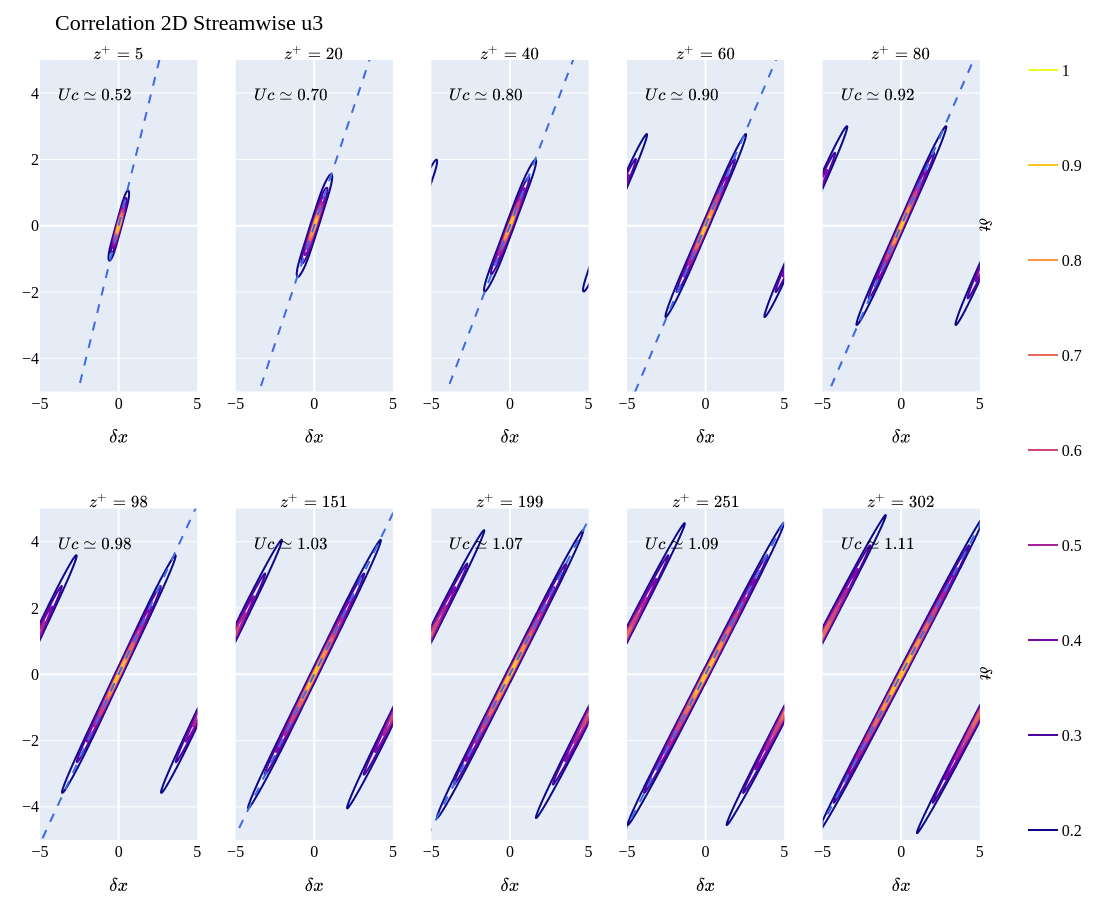
\includegraphics[width=\textwidth]{../../output/figures/channel_wrles_retau395/split_time/frozen_turbulence/correlation2D/u3_all.png}
		\caption{Contour plot of 2D correlation in four streamwise plans. (\textcolor{blue}{- - -}) slop of the ellipses correponding at $\frac{1}{U_c}$. To determine the slop we take the following values of the correlation function: (0.7, 0.8, 0.85, 0.9, 0.95)}
	\end{center}
\end{figure}

\begin{figure}[H]
	\begin{center}
		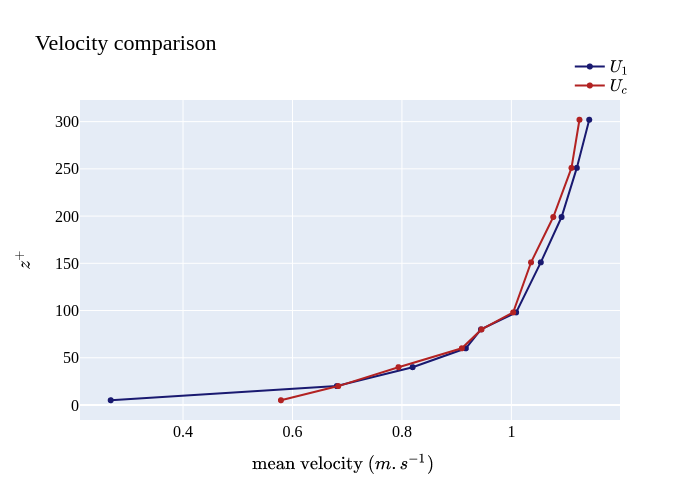
\includegraphics[width=\textwidth]{../../output/figures/channel_wrles_retau395/split_time/frozen_turbulence/correlation2D/u_1c_all.png}
		\caption{Comparion of slop determined velocity ($U_c$) and streamwise mean velocity ($U_1$) in function of $z^+$}
	\end{center}
\end{figure}

\begin{figure}[H]
	\begin{center}
		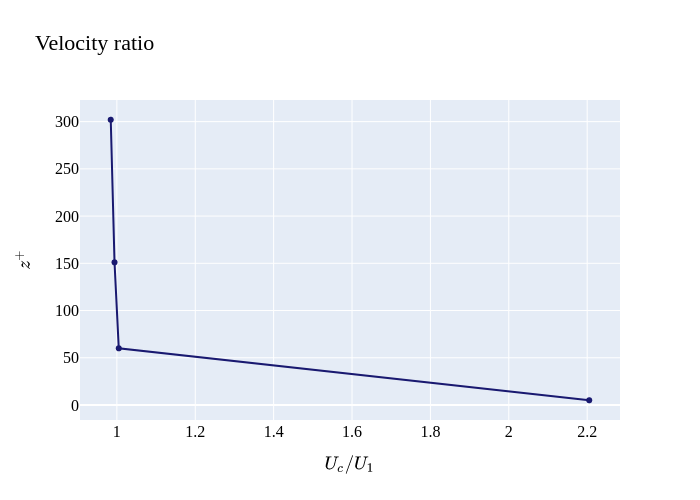
\includegraphics[width=\textwidth]{../../output/figures/channel_wrles_retau395/split_time/frozen_turbulence/correlation2D/u_ratio.png}
		\caption{Ratio of slop determined velocity ($U_c$) and streamwise mean velocity ($U_1$) in function of $z^+$}
	\end{center}
\end{figure}


\subsection{Power spectras}

\begin{figure}[H]
	\begin{center}
		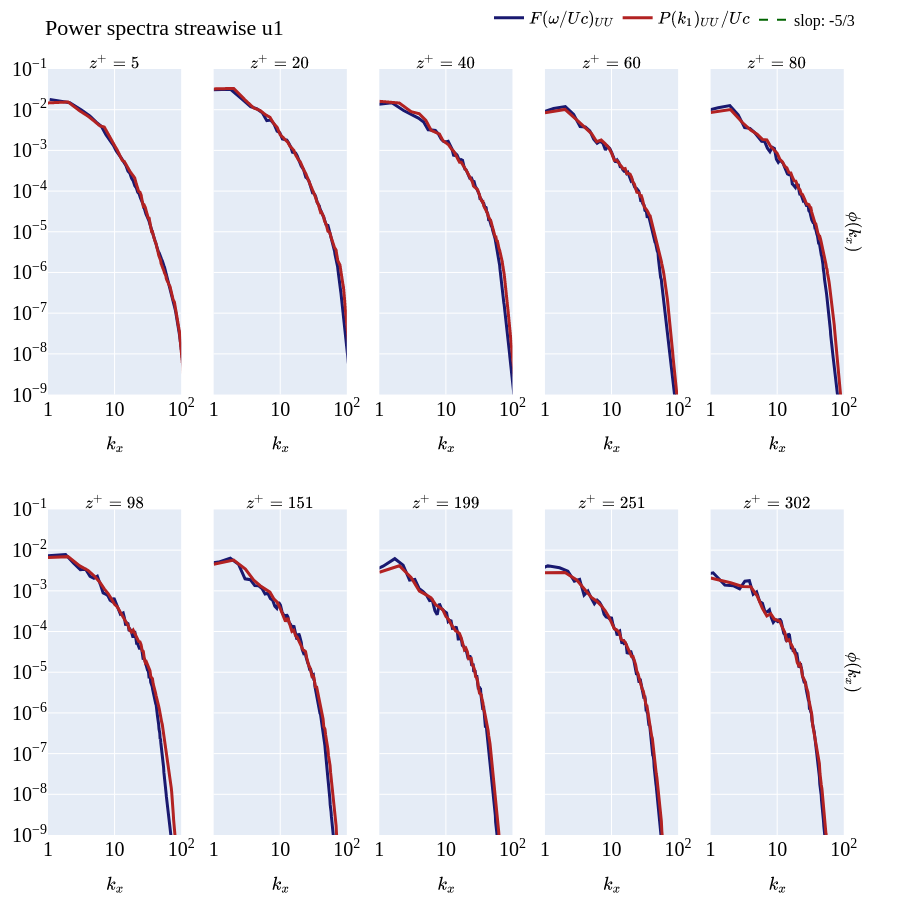
\includegraphics[width=\textwidth]{../../output/figures/channel_wrles_retau395/split_time/frozen_turbulence/power_spectra/u1_all.png}
	\end{center}
\end{figure}

\begin{figure}[H]
	\begin{center}
		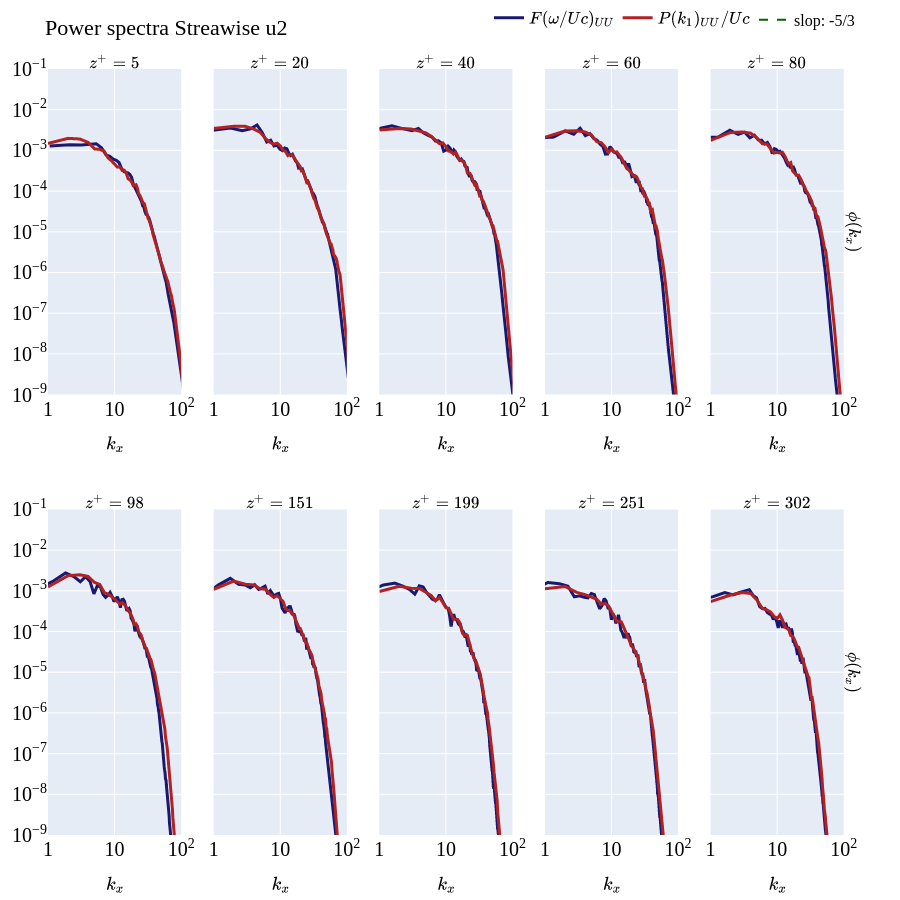
\includegraphics[width=\textwidth]{../../output/figures/channel_wrles_retau395/split_time/frozen_turbulence/power_spectra/u2_all.png}
	\end{center}
\end{figure}

\begin{figure}[H]
	\begin{center}
		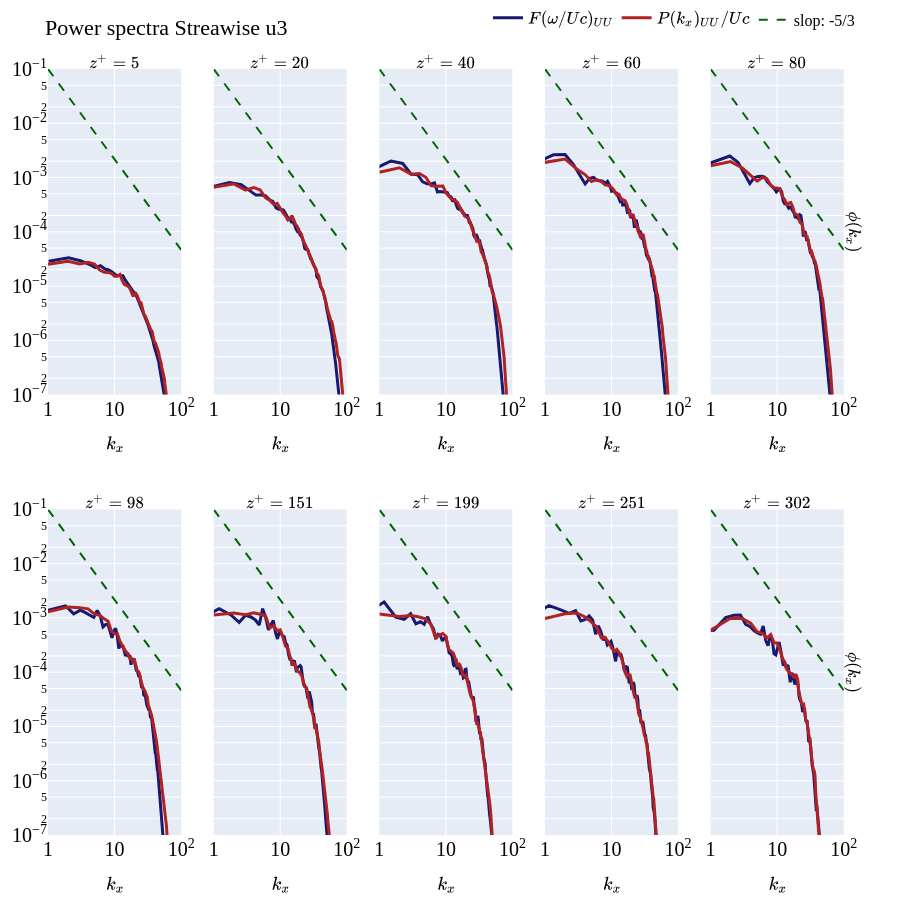
\includegraphics[width=\textwidth]{../../output/figures/channel_wrles_retau395/split_time/frozen_turbulence/power_spectra/u3_all.png}
		\caption{Power spectra in space (red) and time (blue) for the streamwise velocity (top), spanwise velocity (middle) and wall-normal velocity (bottom) at 10 different heights. The Uc took is the mean velocity along the streamwise axis}
	\end{center}
\end{figure}



\section{Spatial correlations}


\begin{figure}[H]
	\begin{center}
		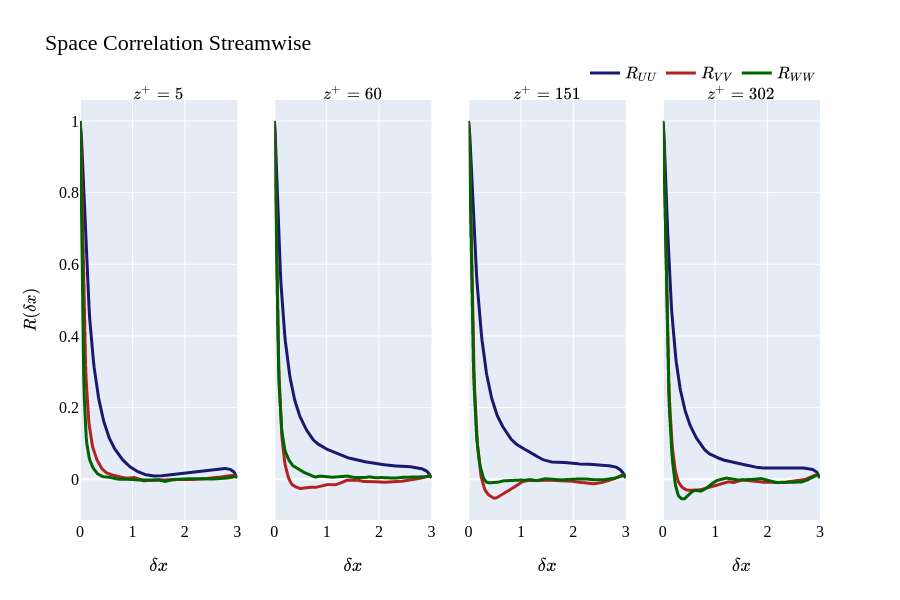
\includegraphics[width=0.9\textwidth]{../../output/figures/channel_wrles_retau395/split_time/space_correlation/streamwise.png}
	\end{center}
\end{figure}

\begin{figure}[H]
	\begin{center}
		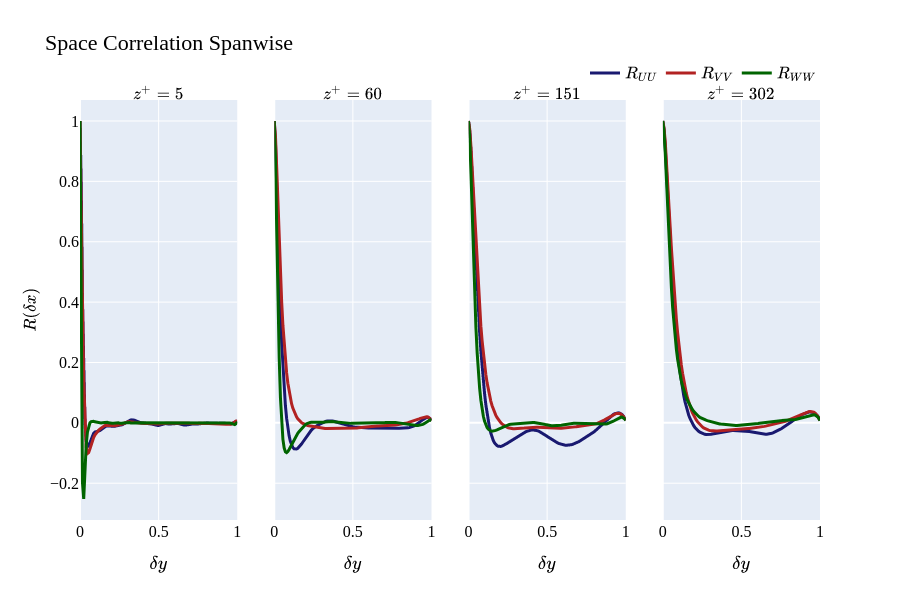
\includegraphics[width=0.9\textwidth]{../../output/figures/channel_wrles_retau395/split_time/space_correlation/spanwise.png}
		\caption{Spatial correllation in a streamwise plan (top figure) and in a spanwise plan (bottom figure). $U$ is the streamwise, $V$ the spanwise and $W$ the wall-normal velocities}
	\end{center}
\end{figure}


\section{Gamma coefficient determination}

\begin{figure}[H]
	\begin{center}
		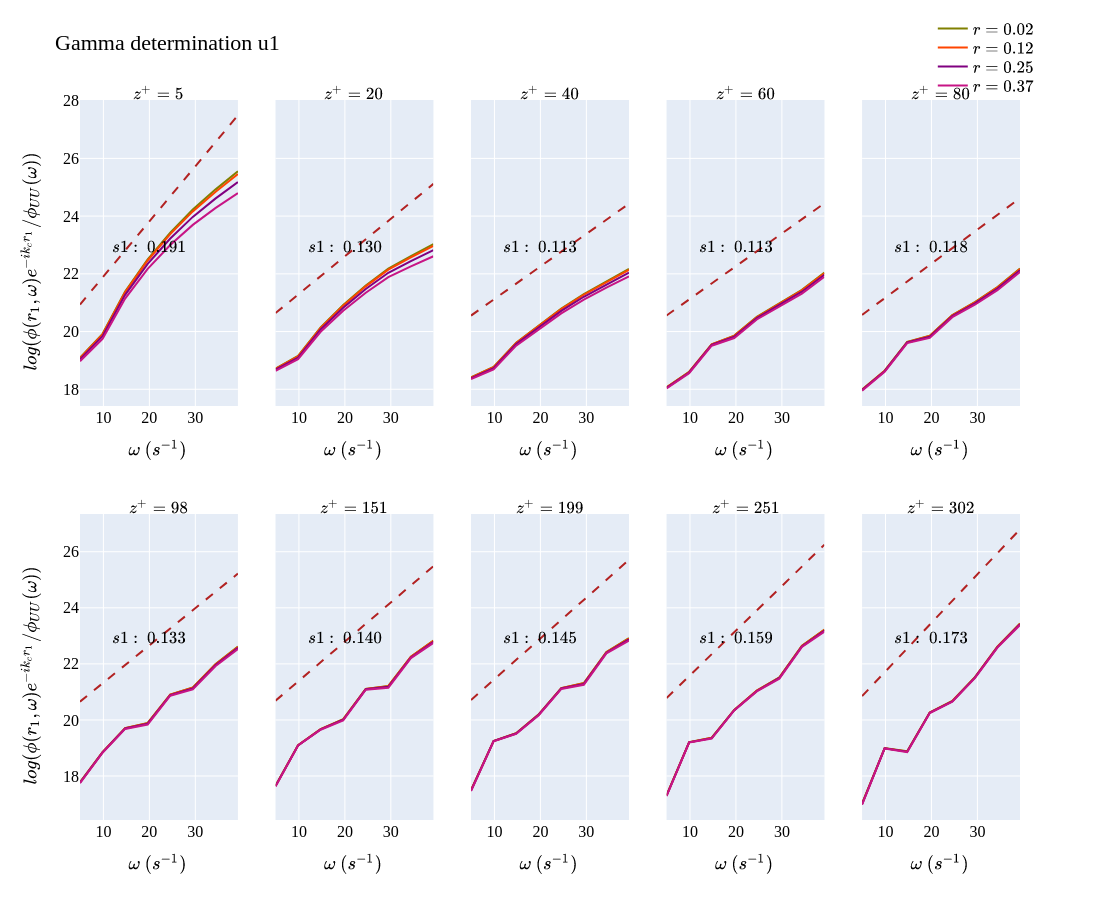
\includegraphics[width=\textwidth]{../../output/figures/channel_wrles_retau395/split_time/gamma/gamma_u1_w_all.png}
	\end{center}
\end{figure}

\begin{figure}[H]
	\begin{center}
		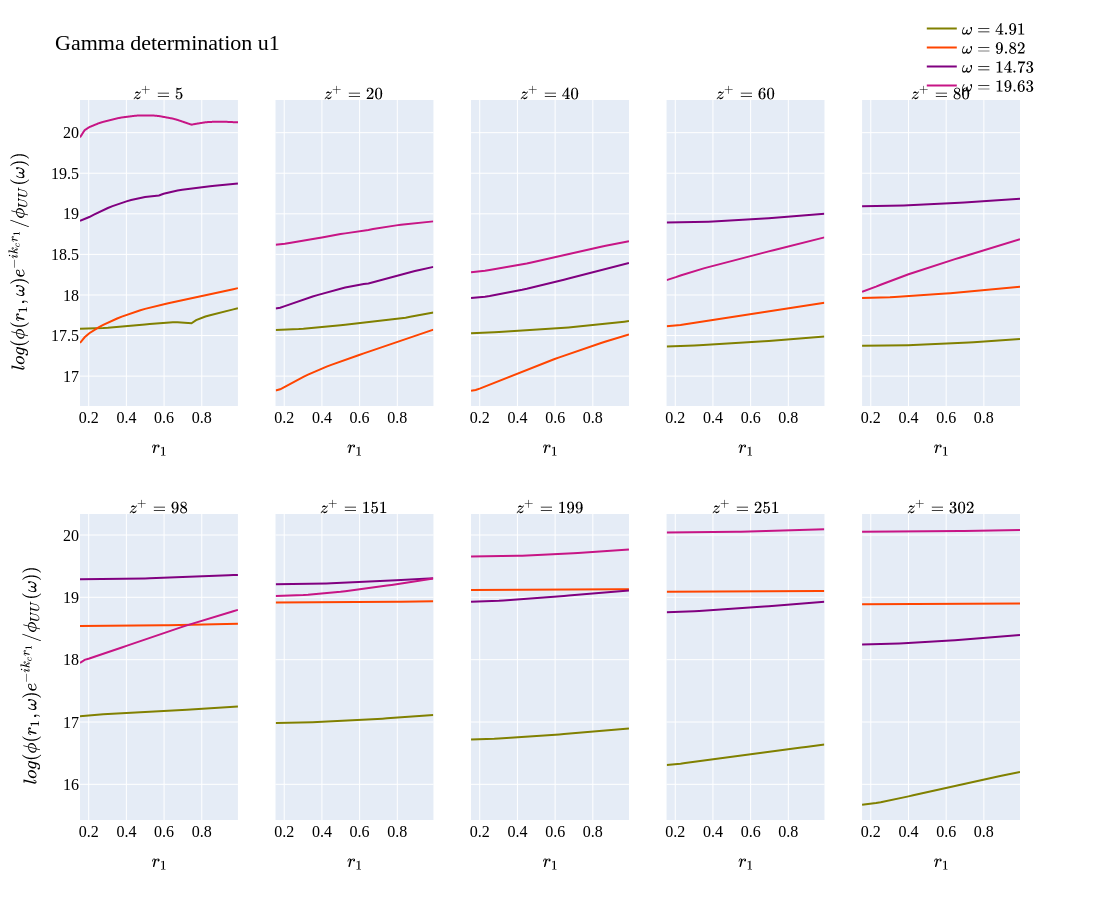
\includegraphics[width=\textwidth]{../../output/figures/channel_wrles_retau395/split_time/gamma/gamma_u1_r_all.png}
	\end{center}
\end{figure}

\begin{figure}[H]
	\begin{center}
		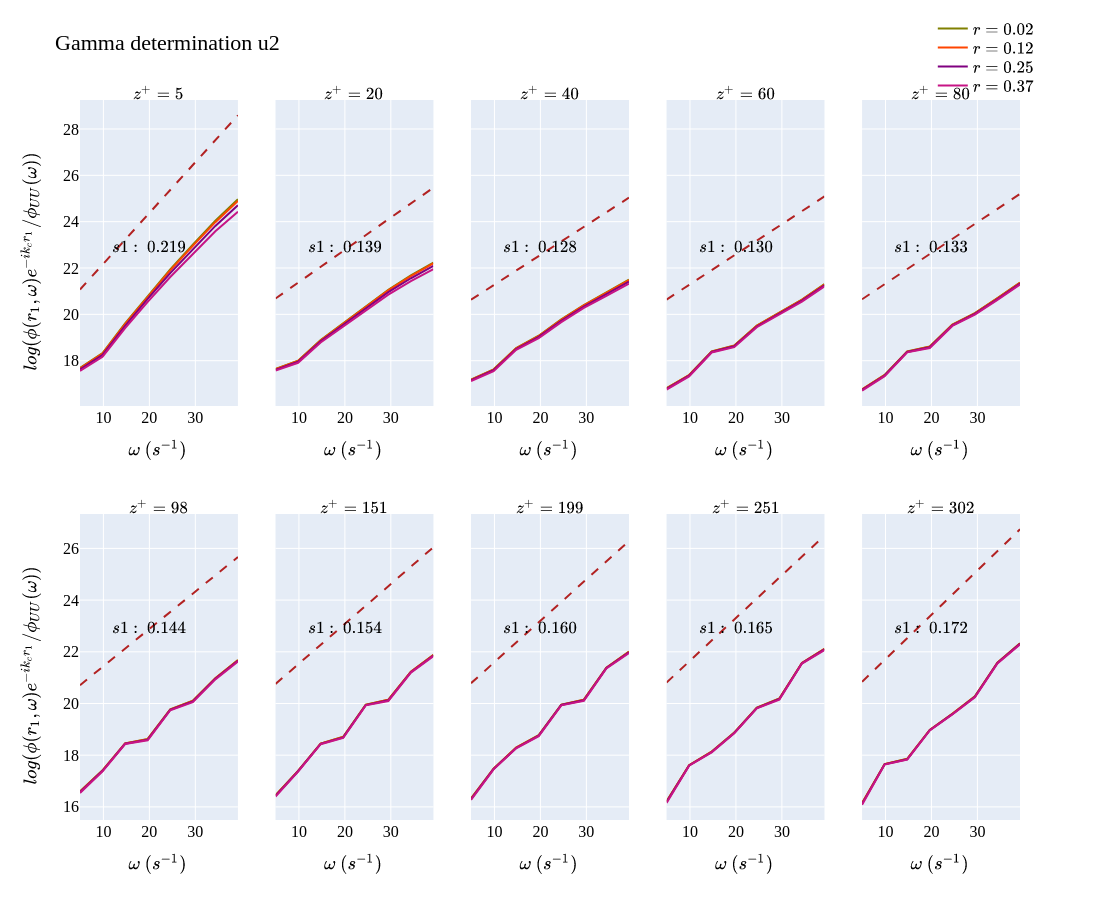
\includegraphics[width=\textwidth]{../../output/figures/channel_wrles_retau395/split_time/gamma/gamma_u2_w_all.png}
	\end{center}
\end{figure}

\begin{figure}[H]
	\begin{center}
		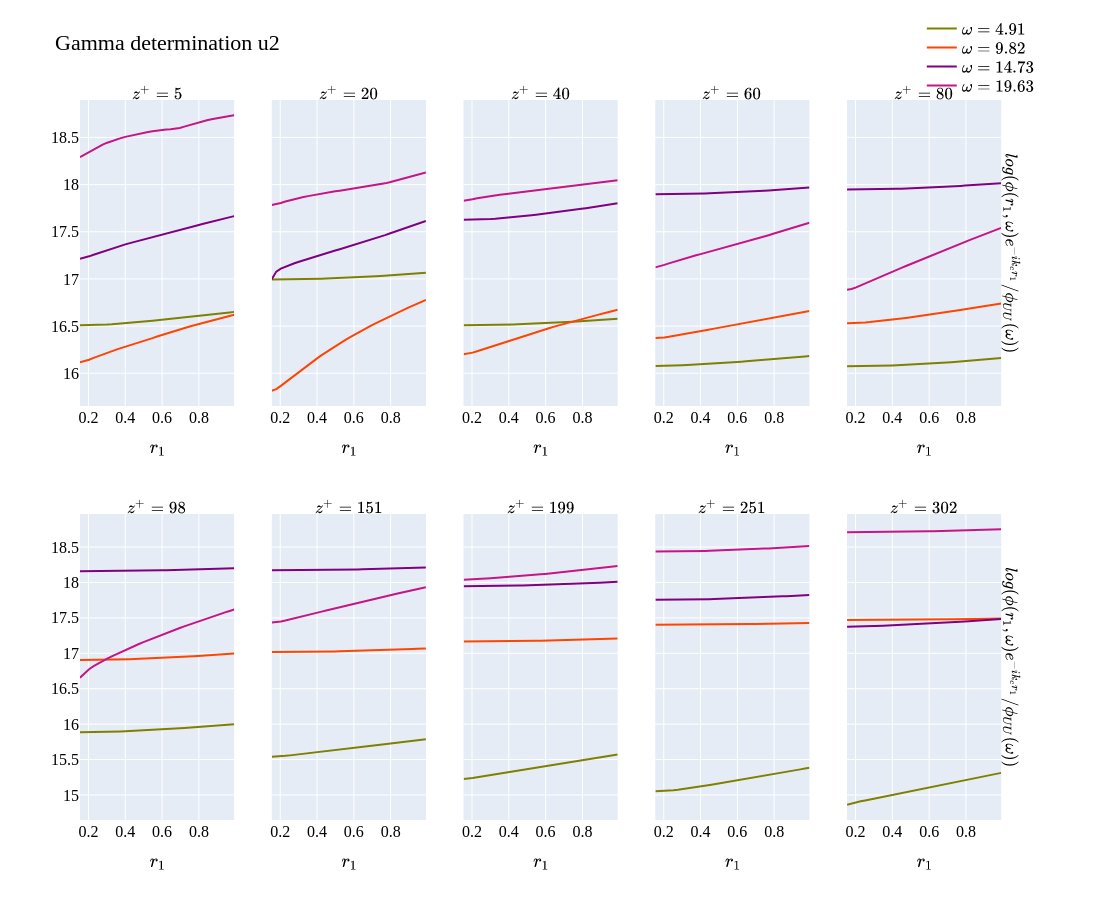
\includegraphics[width=\textwidth]{../../output/figures/channel_wrles_retau395/split_time/gamma/gamma_u2_r_all.png}
	\end{center}
\end{figure}

\begin{figure}[H]
	\begin{center}
		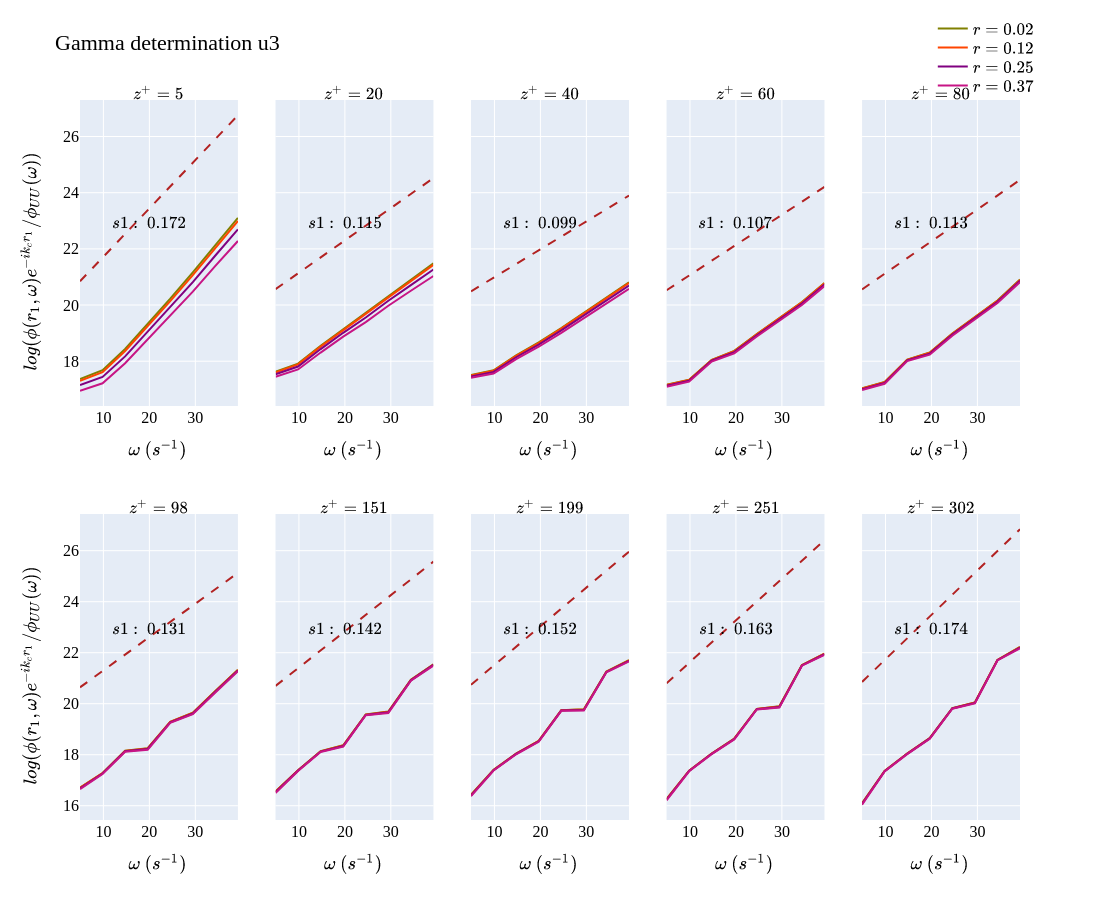
\includegraphics[width=\textwidth]{../../output/figures/channel_wrles_retau395/split_time/gamma/gamma_u3_w_all.png}

	\end{center}
\end{figure}

\begin{figure}[H]
	\begin{center}
		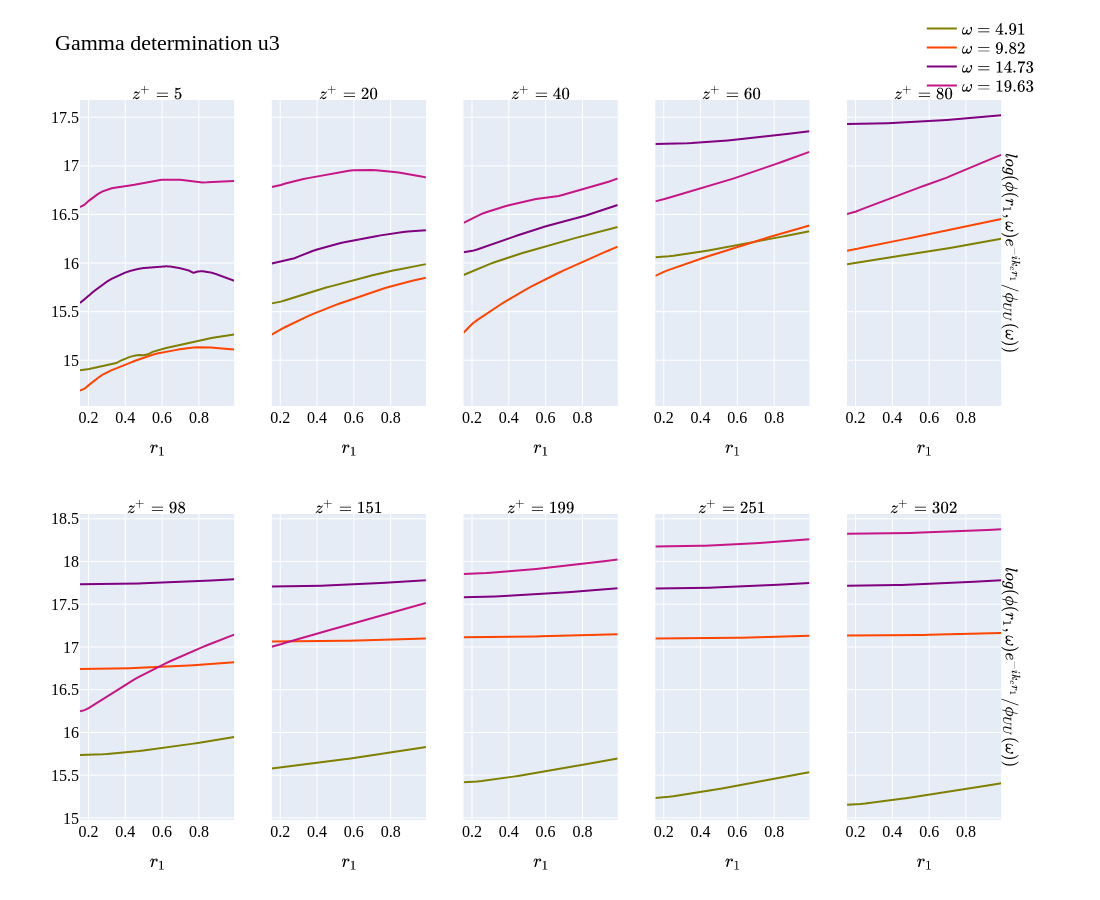
\includegraphics[width=\textwidth]{../../output/figures/channel_wrles_retau395/split_time/gamma/gamma_u3_r_all.png}
		\caption{Determination of $\gamma$ coefficient as $e^{-\gamma k_c r_1} = \frac{\phi(r_1,\omega)}{\phi_{ii}(\omega)}e^{-ik_cr_1}$ ploted in function of $\omega$ or $r$. All these spectra are computed with streamwise plan with streamwise velocity (top figure), spanwise velocity (middle figure) and wall-normal velocity (bottom figure)}
	\end{center}
\end{figure}

\begin{figure}[H]
	\begin{center}
		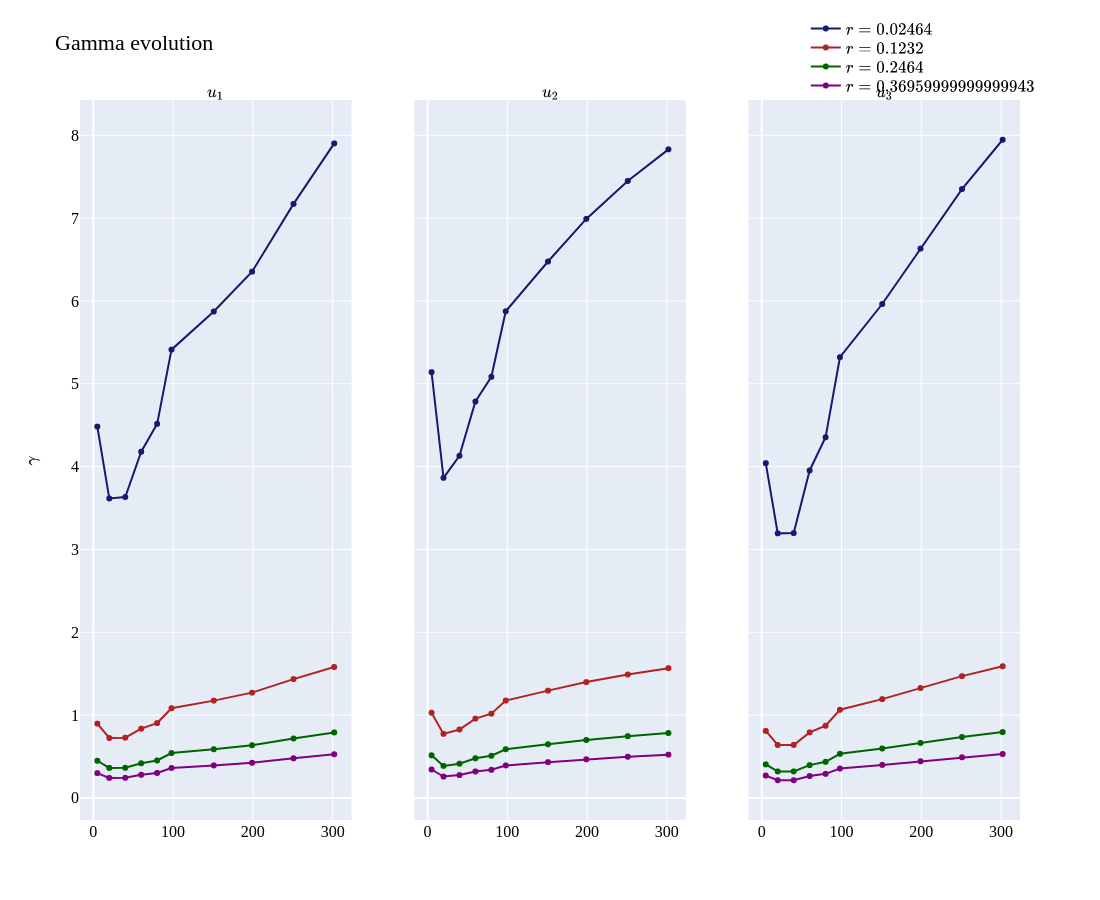
\includegraphics[width=\textwidth]{../../output/figures/channel_wrles_retau395/split_time/gamma/gamma_view_w_all.png}
		\caption{Figure representing the evolution of $\gamma$ coefficient in function of $z^+$ for the $\omega$ dependency, determined by the precedent figures. }
	\end{center}
\end{figure}

\begin{figure}[H]
	\begin{center}
		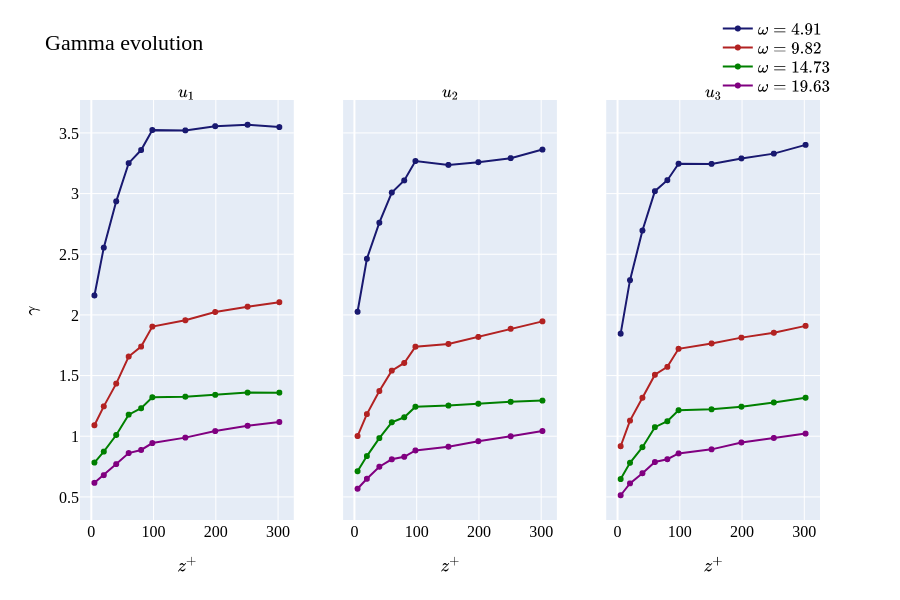
\includegraphics[width=\textwidth]{../../output/figures/channel_wrles_retau395/split_time/gamma/gamma_view_r_all.png}
		\caption{Figure representing the evolution of $\gamma$ coefficient in function of $z^+$ for the $r$ dependency determined by the precedent figures. }
	\end{center}
\end{figure}


\section{Wall-normal plan study}

\begin{figure}[H]
	\begin{center}
		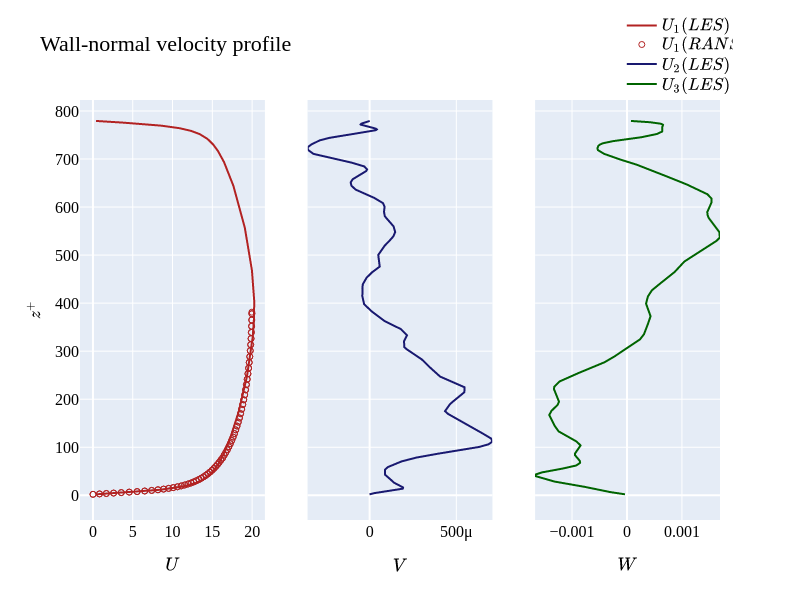
\includegraphics[width=\textwidth]{../../output/figures/channel_wrles_retau395/split_time/Normal_plan/velocity_profiles.png}
		\caption{Mean velocity profile for a normal plan taken at the middle of the channel with 10 wall-normal lignes having 1936 points each.}
	\end{center}
\end{figure}

\begin{figure}[H]
	\begin{center}
		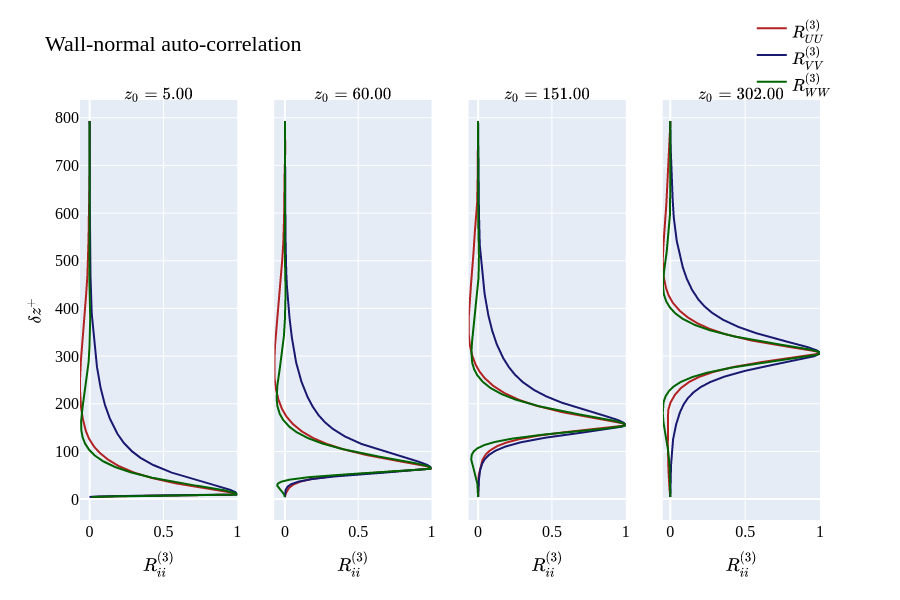
\includegraphics[width=\textwidth]{../../output/figures/channel_wrles_retau395/split_time/Normal_plan/autocorrelation_z.png}
		\caption{Autocorrelation at different height references ($z_0$) for the wall-normal plan.}
	\end{center}
\end{figure}

\begin{figure}[H]
	\begin{center}
		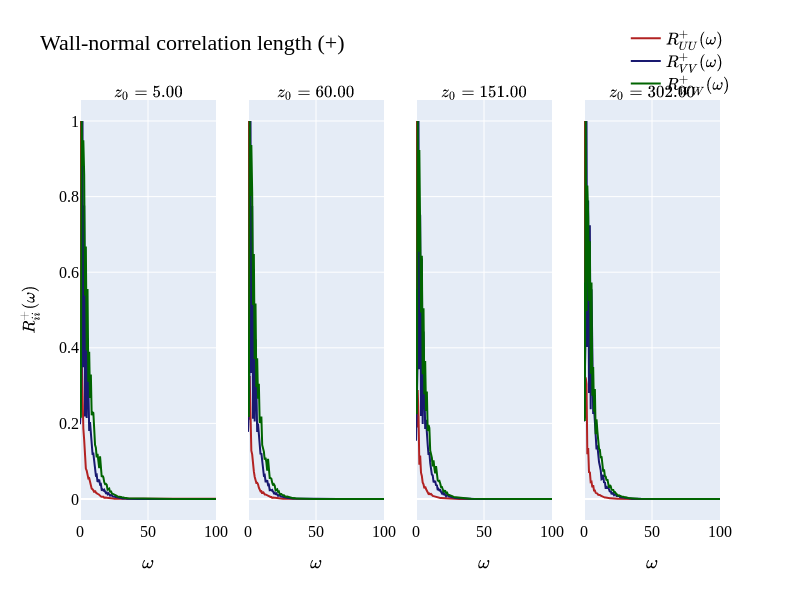
\includegraphics[width=\textwidth]{../../output/figures/channel_wrles_retau395/split_time/Normal_plan/correlation_length_plus.png}
	\end{center}
\end{figure}

\begin{figure}[H]
	\begin{center}
		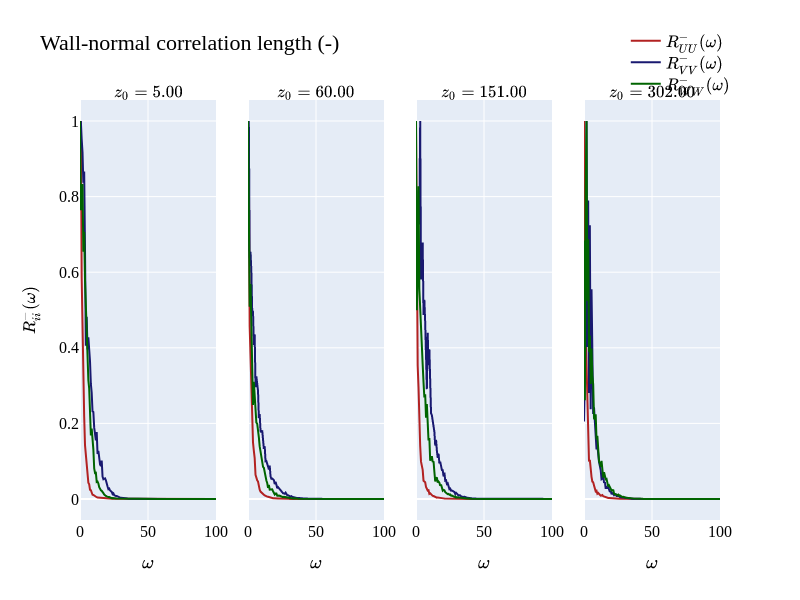
\includegraphics[width=\textwidth]{../../output/figures/channel_wrles_retau395/split_time/Normal_plan/correlation_length_minus.png}
		\caption{Representing the function $R_{ii}^{+/-}(z,\omega)=\int_{\delta z}<u_i(z,\omega)u_i^*(z+\delta z, \omega)>d\delta z$ summed on $z$ and ploted in function o $\omega$}
	\end{center}
\end{figure}


\section{Von Karman}


\begin{figure}[H]
	\begin{center}
		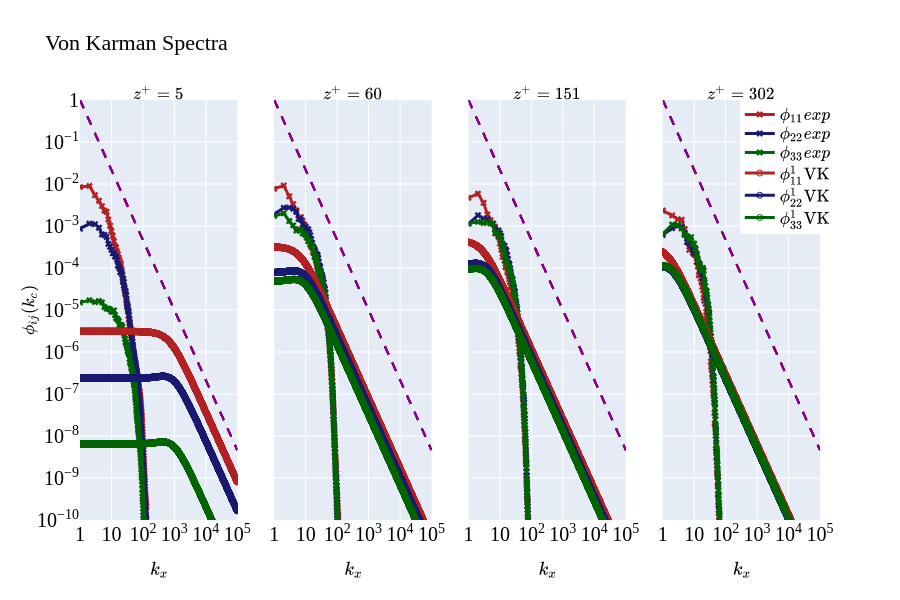
\includegraphics[width=\textwidth]{../../output/figures/channel_wrles_retau395/split_time/von_karman/von_karman_spectra.png}
		\caption{Spectra comparison of LES and DNS datas against von Karman theoretical spectra. The LES spectra have been compute using welch method.}
	\end{center}
\end{figure}

\begin{figure}[H]
	\begin{center}
		\includegraphics[width=\textwidth]{../../output/figures/channel_wrles_retau395/split_time/von_karman/integral_lenght_scale.png}
		\caption{Ratio of integral length scale of spectra for LES datas and von Karman theoretical results. These have been computed by integrating (trapez method) the spectra above.}
	\end{center}
\end{figure}
	
	
\end{document}